%!TEX root = ../Topografia_Relazione_MeoliNicola.tex
\chapter{Fotogrammetria}
Come ultimo esercizio si sono affrontati due progetti di fotogrammetria, consistenti nell'ottenere un'ortofoto di due aree partendo da singole strisciate di foto.

Si illustrerà ora un accenno generale alla fotogrammetria, con l'indicazione dei passaggi effettuati tramite programma \emph{PhotoMod}. 
Si farà poi una carrellata di immagini dei due rilievi, rappresentanti alcuni passaggi e l'ortofoto finale. 

\section{Accenni di fotogrammetria}
La fotogrammetria è quella tecnica grazie la quale è possibile ricostruire posizioni nello spazio a partire da immagini.
Lo fotogrammetria digitale aggiunge alla fotogrammetria tradizionale -- basata sulla lunghezza focale della camera e il formato del sensore -- il fattore della risoluzione delle immagini.

Nei software, dopo aver importato le foto suddivise per strisciate con una certa sovrapposizione tra di esse -- questo serve a non avere ambiguità nel posizionamento del punto nella retta congiungente il centro di proiezione $O$ e il punto immagine $p$ sul piano -- e dopo aver fissato i parametri della camera utilizzata; il procedimento si compone di due passaggi fondamentali: il calcolo dei \textit{Tie Points} e il fissaggio dei \textit{Ground Control Points}.

Il primo consiste in una pre-orientazione delle immagini. 
Il programma (in prima approssimazione) collega tra loro i punti omologhi presenti nei diversi fotogrammi.
Successivamente viene effettuata una verifica dall'operatore degli errori riportati dal programma e, nel caso ce ne sia bisogno, vengono eliminati alcuni di questi punti.
In questo passaggio vengono utilizzate le equazioni di complanarità per legare tra loro i punti omologhi. 
\begin{equation}
	\underline{b}\cdot\left(\underline{\rho_1}\wedge\underline{\rho_2}\right)
\end{equation}
Questo serve ad assicurare che le due rette congiungenti il punto reale $P$ e i due corrispondenti punti sui piani dell'immagine non siano sghembe.
Sono inoltre utilizzate le equazioni di collinearità. 
Esse servono a collegare le coordinate del punto nello spazio oggetto con le coordinate corrispondenti del punto nello spazio immagine.
 

Il secondo passaggio fondamentale consiste nell'assegnazione delle coordinate-oggetto note ai punti presenti in tutti i fotogrammi.

Il programma (dopo vari settaggi quali tipologia di terreno, estensione, precisione, ecc.) rielabora i punti fino ad ottenere una rettifica di tutti i pixel.
Si è venuto così a creare una rappresentazione fedele dei punti dell'ambiente e con le coordinate trasformate di sistema di riferimento  in base ai punti inseriti.
La trasformazione di sistema di riferimento è avvenuta secondo le metodologie elencate nel capitolo \ref{cap:cap3}.
Da questa rappresentazione digitale è infine  possibile creare ed esportare le linee di livello o un'ortofoto.
\section{Primo esempio}
Il primo progetto consisteva in una zona di terreno pianeggiante di circa \SI{2}{\kilo\meter} per lato.  
Per eseguire la procedura si è partiti da 18 foto scattate da una camera posizionata in un aereo, suddivise in tre diverse strisciate.
Particolarità di questo rilievo è che nel terreno sono stati posizionati degli elementi di facile riconoscimento.
Grazie a questi è stato facilmente possibile assegnare le coordinate ai punti omologhi.

In figura \ref{orto1} è riportato una porzione di ortofoto ottenuta dopo l'intera procedura. 
\begin{figure}[htbp]
\centering
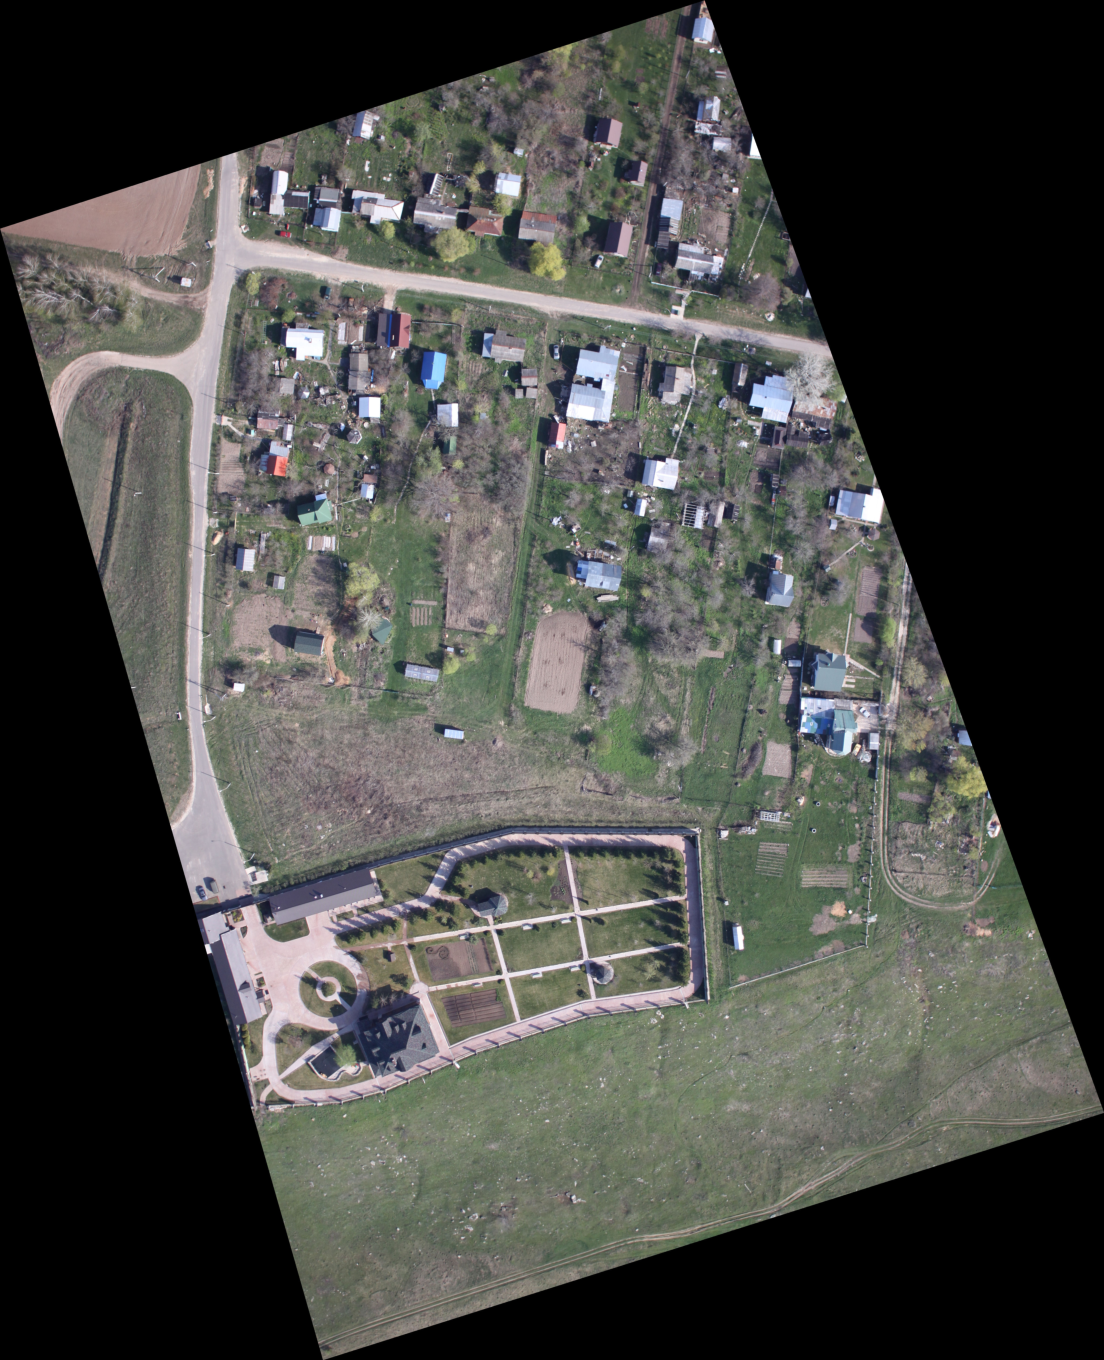
\includegraphics[trim= 3cm 3cm 3cm 3cm,clip,width=0.7\textwidth]{Img/Orto1.pdf}
\caption{Porzione di ortofoto ottenuta dopo la procedura del primo esempio}
\label{orto1}
\end{figure}
%------------------------------------
\section{Secondo esempio} 
Il secondo consisteva in una rappresentazione di una zona montuosa nei pressi di Trento e riportata in un plastico. 
Plastico dalle dimensioni di \SI{1}{\meter} per lato e digitalizzato tramite 8 foto scattate da smartphone.
Data la natura e la grandezza dell'oggetto nella realtà, in questo caso si sono dovuti fare ulteriori settaggi tali da diminuire lo scarto al millimetro o al decimo di millimetro e aumentare così la qualità finale.

Nelle figure sottostanti vengono riportati gli ultimi passaggi della procedura, ovvero la creazione della TIN e della DEM, e la raffigurazione di due ortofoto a risoluzione diversa.
\begin{figure}[htb]
\centering
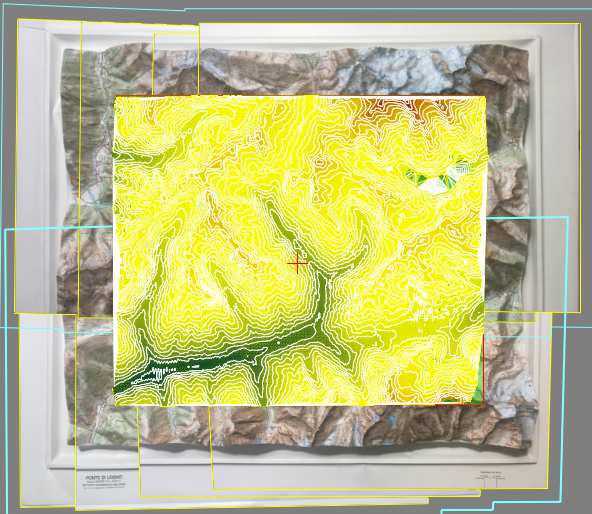
\includegraphics[width=0.6\textwidth,trim=1cm 2cm 1cm 1cm,clip]{Img/TIN.png}
\caption{TIN}
\end{figure}
\begin{figure}[htb]
\centering
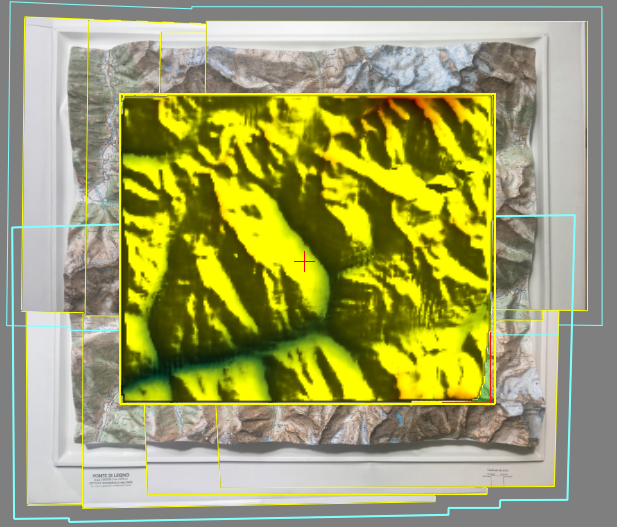
\includegraphics[width=0.6\textwidth,trim=1cm 2cm 1cm 1cm,clip]{Img/DEM.png}
\caption{DEM}
\end{figure}
\begin{figure}[htb]
\centering
\subfloat[][\emph{Precisione del millimetro \label{fig:Orto2_Millimetro}}]
{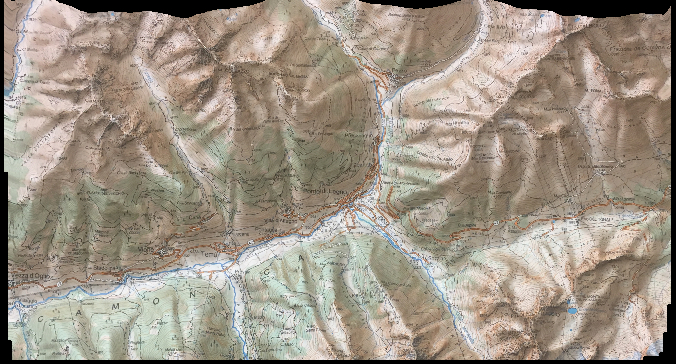
\includegraphics[width=\textwidth,trim=1cm 1cm 1cm 1cm,clip]{Img/Orto2_1.jpg}}
\\
\subfloat[][\emph{Precisione del decimo di millimetro
\label{fig:Orto2_DecimoMillimetro}}]
{\includegraphics[width=\textwidth,trim=3cm 5cm 3cm 5cm,clip]{Img/Orto2_2.jpg}} 
%
\caption{Porzioni di ortofoto ottenute dopo la procedura del primo esempio}
\label{fig:Orto2}
\end{figure} 

